%----------------------------------------------------------------------------
\chapter{Graph neural networks and representation learning}
\label{sec:RepresentationLearning}
%----------------------------------------------------------------------------

\section{Graph neural networks}
%----------------------------------------------------------------------------

Graph Neural Networks (GNNs) are a class of neural networks designed to process and analyze graph-structured data. Unlike traditional neural networks that operate on Euclidean data such as images and text, GNNs work on data represented as graphs, which can capture complex relationships between entities. The importance of GNNs stems from the ubiquity of graph-structured data in various domains:

\begin{itemize}
    \item \emph{Social Networks:} where nodes represent individuals and edges represent relationships or interactions.
    \item \emph{Biological Networks:} such as protein-protein interaction networks, where nodes represent proteins and edges represent interactions.
    \item \emph{Knowledge Graphs:} where nodes represent entities and edges represent relationships between them.
    \item \emph{Infrastructure Networks:} such as transportation and communication networks.
\end{itemize}

GNNs leverage the graph structure to perform tasks like node classification, link prediction, and graph classification, achieving state-of-the-art performance in many applications.
The field of GNNs has seen rapid growth, driven by advances in machine learning and the increasing availability of graph data. Key milestones in the development of GNNs include the introduction of Graph Convolutional Networks (GCNs), Graph Attention Networks (GATs), and various other architectures that have expanded the capabilities and applications of GNNs.

It is essential to understand the basic components of graph structures. Nodes, or vertices, represent entities within the graph, while edges denote the relationships or connections between these nodes. The adjacency matrix is a square matrix used to represent a graph. In this matrix, the element at row $i$ and column $j$ indicates the presence or weight of an edge between nodes $i$ and $j$. This foundational understanding of graph structures is critical for comprehending how GNNs operate on graph-structured data.
Graph data presents unique challenges that differ from traditional \verb+Euclidean data+\footnote{
Euclidean data refers to data that exists within the Euclidean space. It is characterized by having a fixed and regular geometric structure. Examples are images, where data points (pixels) are arranged in a regular grid, and each pixel has a fixed position relative to others and tabular data, where entries are organized in rows and columns within a fixed structure.
}. One primary challenge is its non-Euclidean nature, as graphs lack a fixed geometric structure, making it difficult to apply traditional convolutional neural network (CNN) operations. Additionally, graphs exhibit irregularity, where nodes can have varying numbers of neighbors, unlike pixels in an image which have a fixed number of neighboring pixels. Furthermore, the features of a node in a graph depend not only on the node itself but also on its neighbors and their connections, adding a layer of complexity to the learning process.

In Graph Neural Networks, fundamental operations are important for processing graph data. Message passing enables nodes to exchange information with their neighbors, involving the aggregation of features and subsequent updates to node representations. Aggregation is then employed to combine neighboring node features through operations like mean, sum, or max. Finally, nodes update their representations based on the aggregated information. These operations, although independent, collectively empower GNNs to effectively analyze and process graph data.

Training approaches for Graph Neural Networks encompass diverse methodologies designed for distinct learning paradigms. \cite{DBLP:journals/corr/abs-1812-08434} In supervised learning, GNNs tackle tasks such as node classification, edge prediction, and graph classification. Node classification involves assigning labels to nodes based on their features and connections within the graph. Edge prediction focuses on predicting the existence or properties of edges between nodes. Graph classification aims to classify entire graphs based on their structural and feature characteristics.

In unsupervised learning, GNNs leverage techniques like graph autoencoders and contrastive learning. Graph autoencoders aim to learn meaningful representations of graphs by reconstructing them from compressed embeddings. Contrastive learning involves training the model to distinguish between positive and negative samples, enhancing its ability to capture meaningful patterns in the data.

Semi-supervised learning techniques in GNNs integrate both labeled and unlabeled data to improve performance. By leveraging a combination of labeled data, where nodes or graphs have known labels, and unlabeled data, where labels are absent, semi-supervised learning enables GNNs to generalize better and make predictions on unseen data. \cite{DBLP:journals/corr/KipfW16} These strategies play a pivotal role in enhancing the adaptability and performance of GNNs across various tasks and datasets.

GNNs have revolutionized the field of graph-based machine learning by enabling effective analysis and processing of complex graph-structured data. One key aspect of these networks is node embedding, a technique that involves representing nodes in a graph as low-dimensional vectors in a continuous vector space. Node embedding is the key for capturing the structural and semantic relationships between nodes, allowing GNNs to learn meaningful representations of graph elements. By leveraging node embedding, the network can perform various tasks such as node classification, link prediction, and community detection with improved accuracy and efficiency. This capability to encode graph structures into vector representations enables GNNs to generalize to unseen data and handle large-scale graph datasets, making them a powerful tool for tasks ranging from social network analysis to drug discovery and recommendation systems.


\section{Motivation for representation learning}
%----------------------------------------------------------------------------

In the realm of graph-structured data, the motivation for representation learning lies in the extraction of inner representations in a latent space. These representations serve as compact, semantically rich encodings of the underlying graph structure, enabling their utilization as input to various machine learning algorithms. The key motivations for pursuing such representations are as follows: \cite{DBLP:journals/corr/abs-1709-05584}

\begin{itemize}

    \item \emph{Feature Engineering Simplification:} representation learning alleviates the need for manual feature engineering by automatically generating meaningful representations directly from the graph data. This simplification accelerates the model development process and enhances the scalability of graph-based machine learning tasks.

    \item \emph{Enhanced Generalization:} inner representations in a latent space facilitate enhanced generalization of learned patterns and relationships within the graph data. By capturing the essential characteristics of nodes and edges, these representations enable models to make accurate predictions on unseen data and generalize effectively across diverse tasks.

    \item \emph{Interpretability and Visualization:} the learned representations offer insights into the underlying structure of the graph, enhancing interpretability and enabling intuitive visualization of complex relationships between entities. By mapping nodes to points in a low-dimensional latent space, the inner representations reveal clusters, communities, and structural similarities within the graph.

    \item \emph{Integration with Machine Learning Algorithms:} the compact nature of inner representations makes them ideal inputs for various machine learning algorithms. Whether for classification, regression, or clustering tasks, these representations provide a concise yet informative representation of the graph data, facilitating seamless integration with existing machine learning pipelines.

    \item \emph{Scalability and Efficiency:} representation learning techniques often exhibit scalability and computational efficiency, enabling the analysis of large-scale graph datasets in real-time or near real-time. This scalability is essential for applications across diverse domains, from social network analysis to recommendation systems and beyond.

\end{itemize}

In essence, the motivation for representation learning in the context of graph-structured data centers on the extraction of inner representations in a latent space. When learning representation, an important goal is to produce tabular, low-dimensional embeddings that allow us to infer the structure of the original graph without losing information about it. There are several known methods and algorithms for learning latent representations, two of the most common of which, DeepWalk and node2vec, are discussed in this thesis.

\section{DeepWalk} 
%----------------------------------------------------------------------------

DeepWalk is an approach for learning latent representations of vertices in a network. Introduced by $Perozzi$, $Al-Rfou$, and $Skiena$ in their 2014 paper \cite{DBLP:journals/corr/PerozziAS14} this method applies the concept of word embeddings, used in natural language processing, to graph structures. 
In social networks and other graph-based data structures, understanding the relationships between nodes is crucial. Traditional graph analysis methods, like centrality measures and community detection algorithms, often fail to scale or generalize to large, dynamic graphs. DeepWalk addresses these limitations by providing a scalable, unsupervised learning technique that captures the structural properties of a graph through node embeddings while preserving neighborhood similarity and community structure.

DeepWalk uses local information obtained from truncated random walks to learn latent representations by treating walks as the equivalent of sentences and nodes as the words. By simulating random walks, the algorithm effectively captures the local and global structure of the graph.

Once the random walks are generated, DeepWalk uses the Skip-Gram model \cite{DBLP:journals/corr/MikolovSCCD13} from natural language processing to learn the embeddings. The Skip-Gram model aims to maximize the probability of predicting a node's neighbors within a window in the random walk, thus embedding nodes that frequently co-occur in similar contexts. The DeepWalk algorithm consists of several key steps which according to the paper are:

\begin{enumerate}
   
    \item \emph{Random walk generation:} for each node, simulate multiple random walks of fixed length.
    \item \emph{Context window creation:} for each node in a walk, create context windows of a specified size.
    \item \emph{Skip-Gram training:} use the Skip-Gram model to maximize the co-occurrence probability of nodes within the context windows.
    \item \emph{Embedding learning:} update the embeddings iteratively using \verb+stochastic gradient descent.+\footnote{An optimization algorithm used in machine learning to minimize a loss function by iteratively updating model parameters using randomly selected subsets (mini-batches) of the training data.}
\end{enumerate}

DeepWalk optimizes the objective function \ref{dw_opt_func} 
which maximizes the sum of the logarithmic probabilities of node $u$ given node $v$, over all nodes $v$ in the set of vertices $V$ and their neighborhoods ${N(v)}$, parameterized by $\Theta$,
where  $\Theta$ represents the embedding parameters.


\begin{align}
\label{dw_opt_func}
\max_{\Theta} \sum_{v \in V} \sum_{u \in N(v)} \log P(u \mid v; \Theta)
\end{align}

The hyperparameters of the algorithm include the length of random walks, which determines how far the walk can explore from the starting node, and the number of walks per node, which influences the coverage and diversity of the training data. Additionally, the window size defines the context window for the Skip-Gram model, specifying how much of the neighborhood is considered during training. Lastly, the embedding dimension sets the size of the latent representation for each node, affecting the level of detail in the learned embeddings. DeepWalk is efficient, with time complexity approximately linear in the number of edges and the length of the random walks. This efficiency makes it suitable for large-scale graphs.

\begin{figure}[ht!]
	\centering
        \vspace{0.5cm}
        \begin{subfigure}[b]{0.45\columnwidth}
                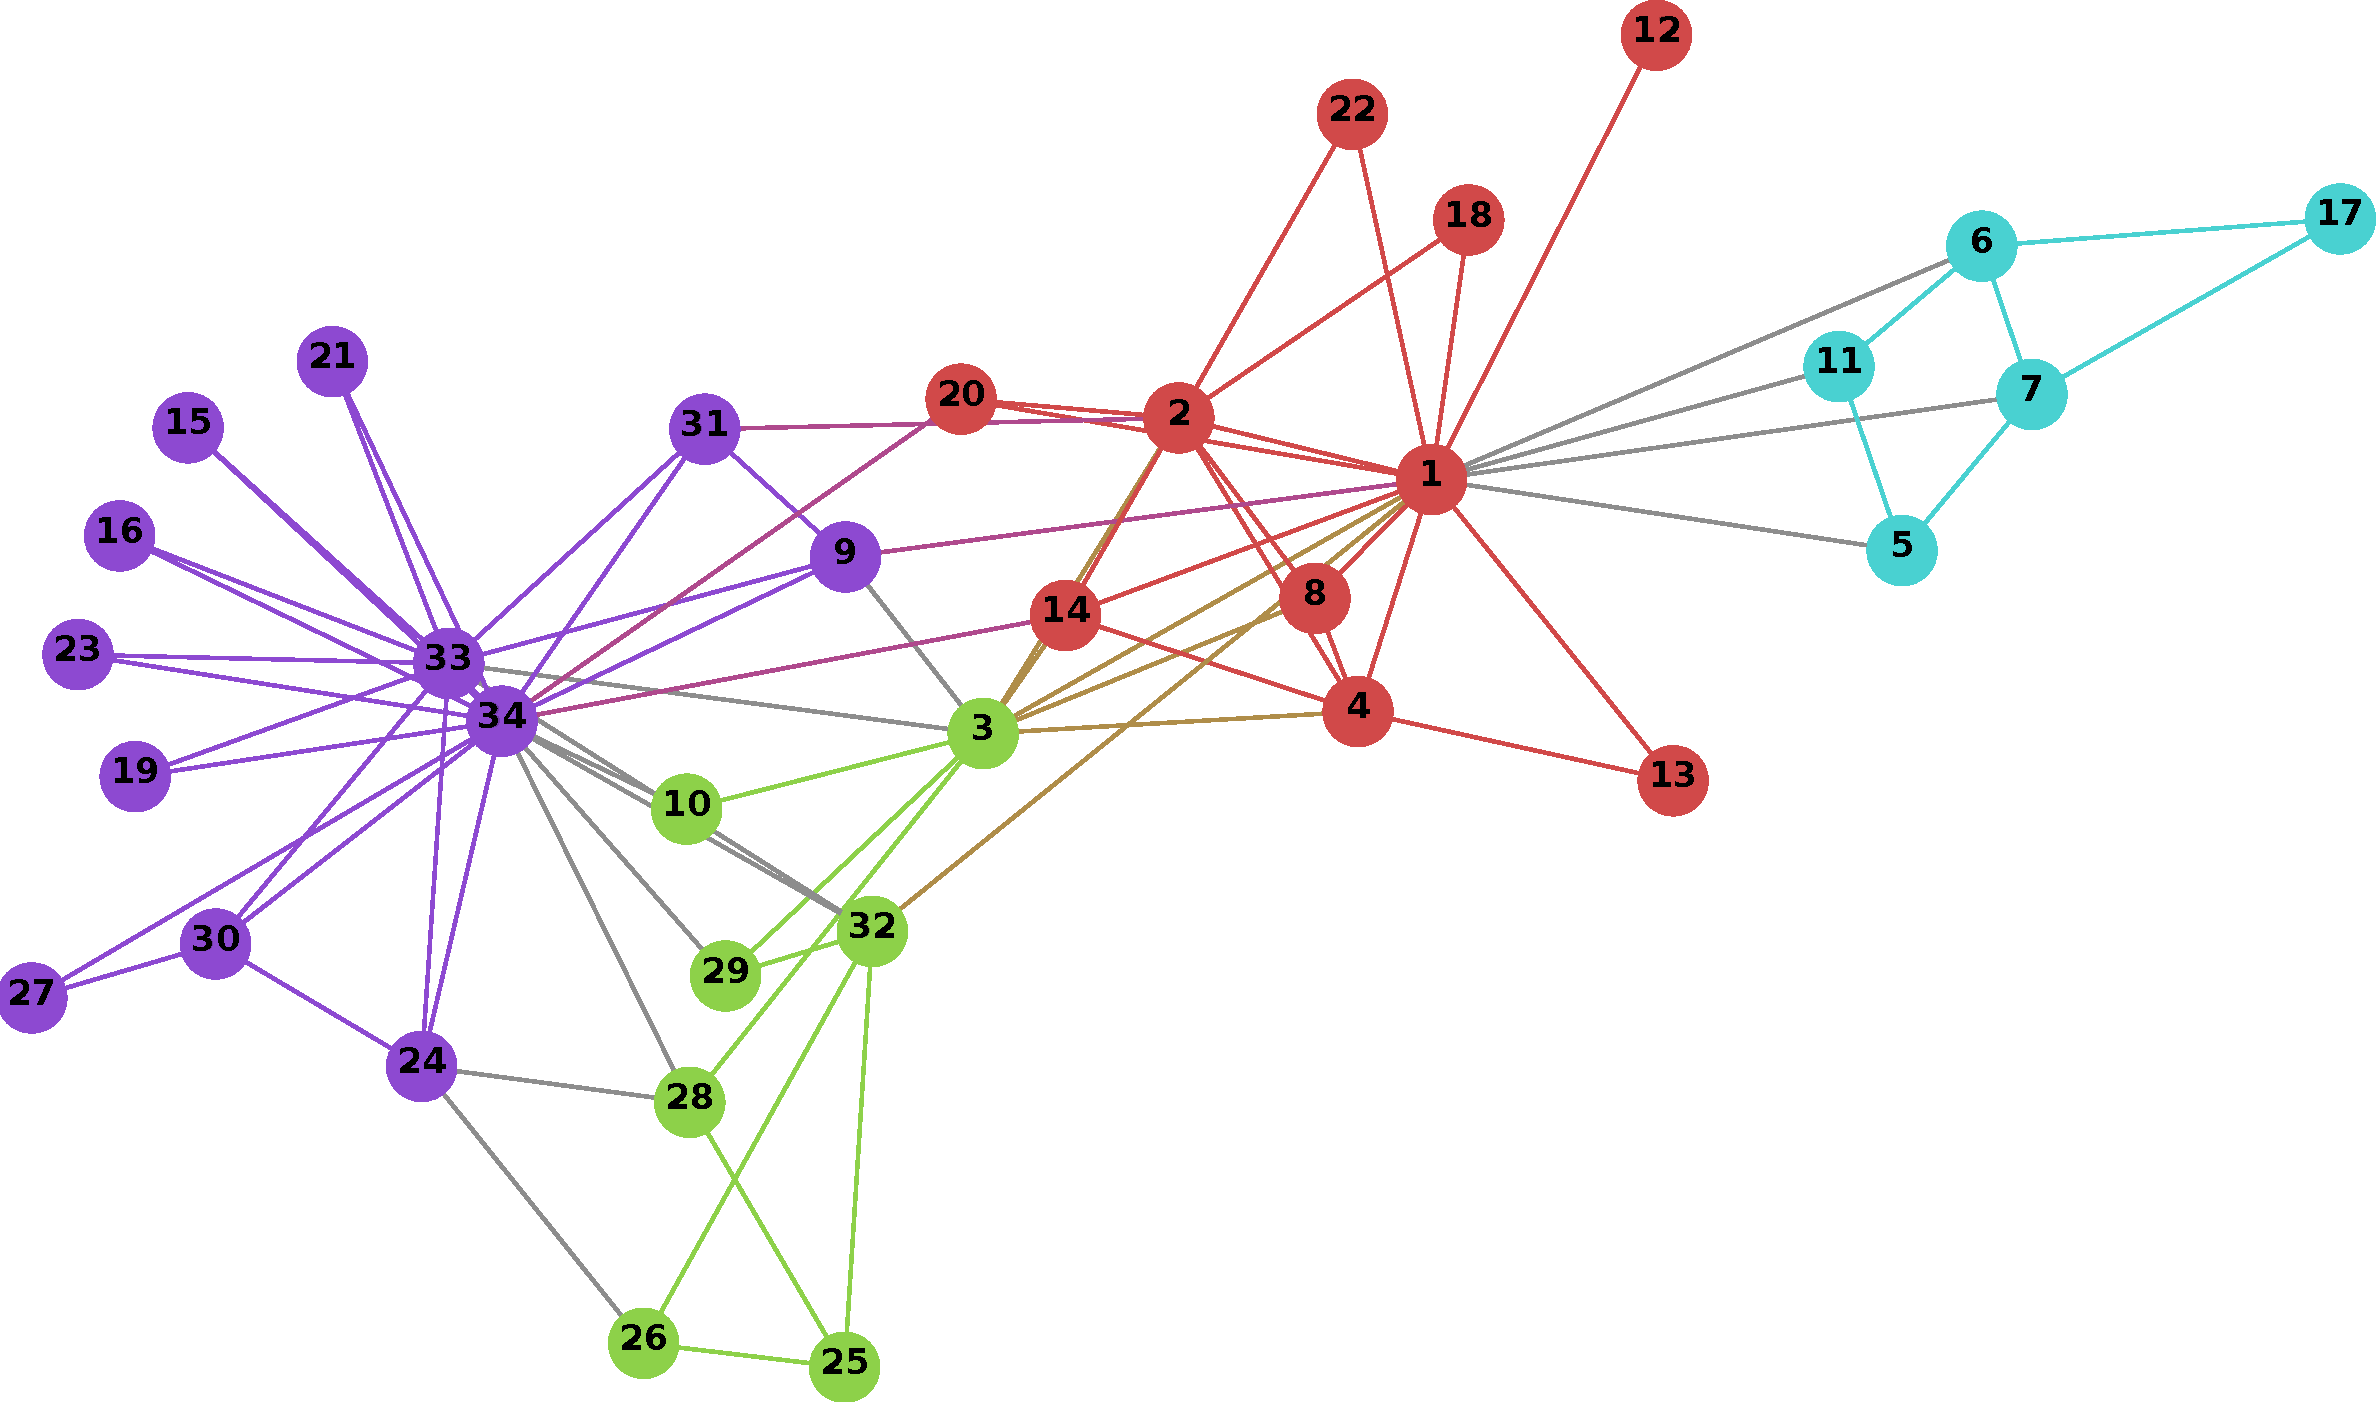
\includegraphics[width=\columnwidth]{figures/karate_graph.pdf}
                \caption{Input: Karate Graph}
                \label{fig:toy_example_graph}
        \end{subfigure}
        \begin{subfigure}[b]{0.45\columnwidth}
                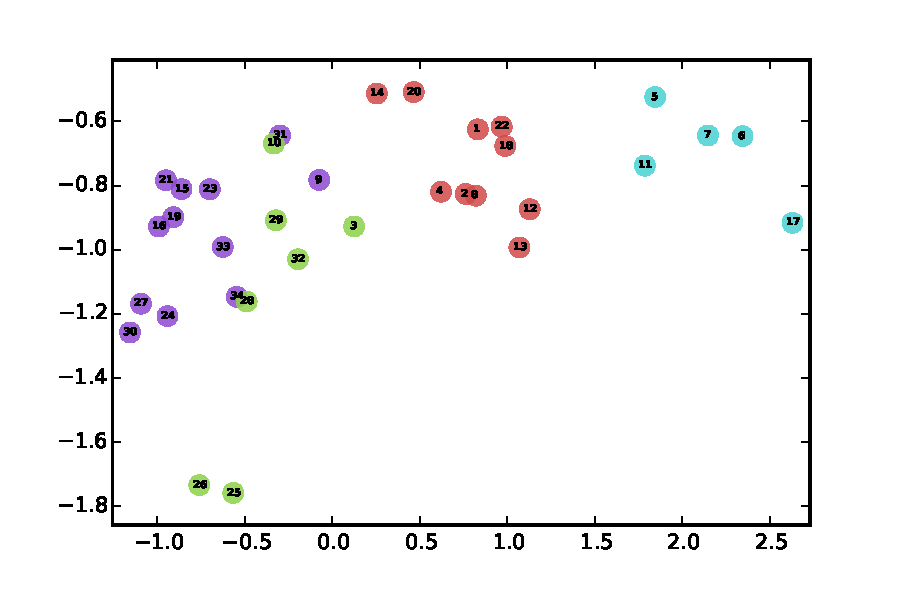
\includegraphics[width=\columnwidth]{figures/karate.pdf}
                \caption{Output: Representation}
                \label{fig:toy_example_embedding}
        \end{subfigure}
        \vspace{0.25cm}
        \caption{
		As presented in the original article the input-output pair on the Karate Graph. The input (a) is a graph representation with nodes and edges, the output (b) is a set of $\mathbb{R}^2$ vectors (representations) in the latent space. In higher dimensions, this kind of visualization is not possible directly.
        }
        \vspace{0.5cm}
        \label{fig:toy_example}
\end{figure}

The DeepWalk algorithm offers several advantages, including scalability, as it is suitable for large graphs due to its linear complexity. It also benefits from being an unsupervised learning method, which means it does not require labeled data for training. Additionally, DeepWalk is flexible and can be applied to various types of graphs and tasks. However, the algorithm has some limitations, such as sensitivity to the choice of hyperparameters, which can significantly impact performance. Moreover, it primarily captures local structures within the graph, which may be a drawback for tasks that require a more comprehensive understanding of global structural properties. 

This method represents a significant advancement in the field of graph representation learning. By leveraging techniques from natural language processing, it provides a scalable and effective method for embedding nodes in a graph, preserving both local and global structures. The algorithm's success in various applications underscores its utility and potential for further development and adaptation in more complex and diverse graph-based scenarios.


\section{Node2vec algorithm}
%----------------------------------------------------------------------------
DeepWalk uses uniform random walks to explore the graph, treating each step as an equal probability transition to any of the neighboring nodes. While this approach effectively captures local node neighborhoods and works well for many tasks, it has limitations. Uniform random walks do not differentiate between different types of graph structures, treating all transitions equally. This can lead to suboptimal representations for nodes in complex graphs. They also primarily capture local structures, such as immediate neighborhoods. These uniform random walks may not effectively capture more global structures or diverse node roles in the graph. 

Node2vec is an advanced algorithm for learning continuous feature representations for nodes in a graph, introduced by $Aditya Grover$ and $Jure Leskovec$ in their 2016 paper.\cite{DBLP:journals/corr/GroverL16} Building upon the foundations laid by DeepWalk, node2vec enhances the flexibility and capability of graph-based embeddings by introducing a more sophisticated random walk strategy that balances local and global network structures. Node2vec employs a flexible biased random walk strategy that interpolates between breadth-first search (BFS) and depth-first search (DFS). This is controlled by two hyperparameters: 
$p$ and $q$. The return parameter $p$ controls the likelihood of immediately revisiting a node, promoting exploration of new nodes. The in-out parameter $q$ determines the likelihood of visiting nodes further away, balancing between BFS (local neighborhood) and DFS (global exploration), as shown in Figure~\ref{strategies}

\begin{figure}[ht!]
	\centering
        \vspace{0.5cm}
	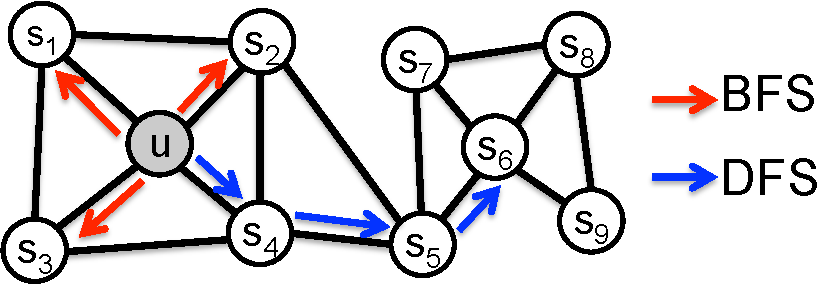
\includegraphics[width=0.90\textwidth]{figures/bfsdfs}
        \vspace{0.25cm}
	\caption{Search strategies from node $u$ if $walkLength=3$.}
	\label{strategies}
        \vspace{0.5cm}
\end{figure}

Similar to DeepWalk, node2vec uses the Skip-Gram model to maximize the probability of observing context nodes given a target node within the biased random walks. This helps in learning embeddings that preserve node neighborhoods effectively. The algorithm introduces several hyperparameters next to $p$ and $q$ that enhance its flexibility and effectiveness: 

\begin{itemize}
    \item \emph{Length of random walks:} determines how far the walk can explore from the starting node, influencing the capture of structural information.
    \item \emph{Window size:} defines the context window for the Skip-Gram model, specifying how many neighboring nodes to consider during training.
    \item \emph{Embedding dimension:} specifies the size of the latent representation for each node, affecting the granularity of the learned embeddings.
    \item \emph{Number of walks per node:} affects the coverage and diversity of the training data, ensuring comprehensive exploration of the graph.
\end{itemize}

Following the definition of the hyperparameters, the node2vec algorithm can be outlined through several key steps. The pseudo algorithm of node2vec is described in Algorithm~\ref{n2v_alg}.

\begin{algorithm}[h]
\vspace{0.5cm}
\caption{node2vec}
\begin{algorithmic}[1]
\State \textbf{Input:} Graph $G = (V, E)$, walk length $l$, number of walks per node $r$, context size $k$, return parameter $p$, in-out parameter $q$, embedding dimension $d$
\State \textbf{Output:} Node embeddings $\Theta$
\State Initialize embeddings $\Theta$ randomly
\Function{BiasedRandomWalk}{$G, v, l, p, q$}
    \State $walk \gets [v]$
    \For{$i = 1$ to $l - 1$}
        \State $curr \gets walk[-1]$
        \State $neighbors \gets \text{Neighbors}(G, curr)$
        \State $probabilities \gets \text{ComputeTransitionProbabilities}(curr, neighbors, p, q)$
        \State $next \gets \text{Sample}(neighbors, probabilities)$
        \State \text{Append} $next$ \text{to} $walk$
    \EndFor
    \State \textbf{return} $walk$
\EndFunction
\State $W \gets []$ \Comment{List to store all walks}
\For{each node $v \in V$}
    \For{$i = 1$ to $r$}
        \State $W_v \gets \text{BiasedRandomWalk}(G, v, l, p, q)$
        \State \text{Append} $W_v$ \text{to} $W$
    \EndFor
\EndFor
\State \text{Train the Skip-Gram model using walks $W$ to learn embeddings $\Theta$}
\State \textbf{return} $\Theta$
\end{algorithmic}
\label{n2v_alg}
\vspace{1.0cm}
\end{algorithm}

Initially, for each node in the graph, multiple random walks of a specified length are generated using a biased random walk strategy, controlled by the return parameter 
$p$ and the in-out parameter 
$q$. These parameters guide the walk to balance between exploring local neighborhoods and traversing further into the graph, effectively capturing both local and global structures. The generated walks are then used to create context windows for each node, which serve as training samples for the Skip-Gram model. It is trained to maximize the likelihood of observing context nodes given a target node, iteratively updating the node embeddings through stochastic gradient descent.

Node2vec offers better latent representation of node roles by effectively identifying and representing nodes with similar structural roles but located in different parts of the graph. This is helpful for tasks like role discovery and anomaly detection. Additionally, the ability to control the walk’s exploration pattern allows node2vec to capture context-specific features of nodes, improving the quality of embeddings for downstream tasks.

By varying the parameters $p$ and $q$, we can control the information compression of the embeddings about the relations of the graph. With a stronger BFS strategy, it highlights the adjacency clusters of the graph, i.e. a vertex will be similar to its neighbours in the latent space. (homophily) If the DFS strategy is stronger, the algorithm captures the global role of vertices in the graph structure. (structural equivalence). By performing classification with embeddings at the vertices of the original graph, we can see an example of the two extreme cases of the mixed discovery strategy on Figure~\ref{strategies_visual}.

\begin{figure}[ht!]
	\centering
	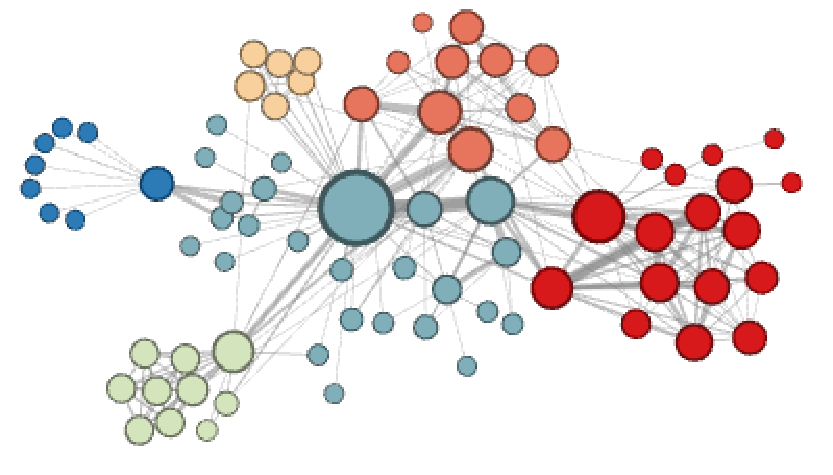
\includegraphics[width=0.70\textwidth]{figures/homo}
	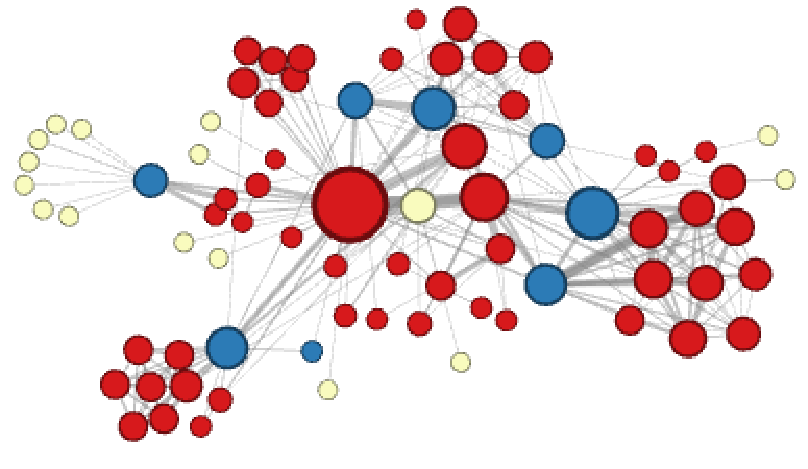
\includegraphics[width=0.70\textwidth]{figures/struceq}
	\caption{The two extreme cases of exploration strategy visualized on Les Mis\'{e}rables coappearance network with node classifying, from the original paper.\cite{DBLP:journals/corr/GroverL16} Homophily on top and structural equivalence at the bottom.}
        \label{strategies_visual}
\end{figure}

The nuanced node embeddings generated by node2vec lead to better performance in node classification tasks, as they capture more detailed structural information. For link prediction, node2vec improves the accuracy by considering both local and global structures. Furthermore, the flexible walk strategy enhances the ability to detect communities, effectively capturing both tight-knit groups and broader community structures. The original paper \cite{DBLP:journals/corr/GroverL16} demonstrates through extensive experiments on various benchmark datasets that biased random walks significantly improve the quality of node embeddings. 

The introduction of biased random walks in node2vec represents a substantial advancement over the uniform random walks used in DeepWalk. By allowing the algorithm to balance between local and global graph exploration, node2vec can capture a more diverse set of structural patterns and node roles. This flexibility translates into better performance across a wide range of applications, making node2vec a more powerful tool for network analysis.